\section{Example showing the importance of causal analysis over historical commits} \label{app:commit-importance}

\noindent\textbf{Figures~\ref{fig:code_a}--\ref{fig:code_c}:}
Illustration of \cresearcher{} analyzing and repairing a real-world memory leak bug\footnote{Bug in Syzbot dashboard: \url{https://syzkaller.appspot.com/bug?id=92a742e993c8b9e769f8502a0497c88c0afa78af}.} from the \kbenchsyz{} dataset~(the complete trajectory of \cresearcher{} is truncated and only the relevant parts are shown due to space constraints).
Figure~\ref{fig:code_a} shows the developer’s original commit, including the fix and a "Fixes:" tag that references the buggy commit where the issue originated: commit \colorbox{highlightyellow}{\texttt{6679f4c5e5a6}}—highlighted in yellow. This section is shown in the \textcolor{black}{\fcolorbox{black}{orangebox}{orange box}}. The developer's fix is available at the following link\footnote{Developer’s fix commit: \url{https://git.kernel.org/pub/scm/linux/kernel/git/torvalds/linux.git/commit/?id=50d34a0d151dc7abbdbec781bd7f09f2b3cbf01a}.}. Figure~\ref{fig:code_b} displays a subset of actions taken by \cresearcher{} in the \analysisphase{} phase, specifically several \texttt{search\_commits} steps (\textcolor{black}{\fcolorbox{black}{greenbox}{green box}}), which reveal how the agent retrieves both the buggy commit and other related commits that involve memory management. These retrieved historical commits provide guidance in the \synthesisphase{} phase. Figure~\ref{fig:code_c} presents the patch and analysis synthesized by \cresearcher{} (\textcolor{black}{\fcolorbox{black}{bluebox}{blue box}}) during the \synthesisphase{} phase, which correctly identifies the missing deallocation and inserts the appropriate \texttt{kfree(bt\_const\_extended)} call. Notably, \cresearcher{} successfully navigates to the same buggy commit identified by the developer’s "Fixes:" tag, demonstrating its ability to infer causality and leverage prior commits to localize and fix bugs.

\begin{figure}[H]
    \centering
    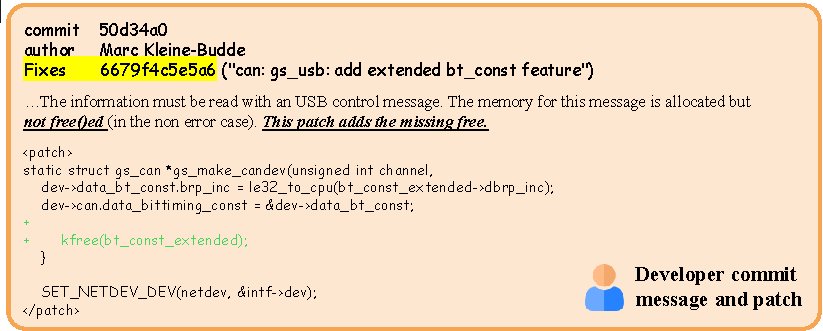
\includegraphics[width=\linewidth]{images/commit-importance-a.pdf}
    \caption{Developer commit message and patch.}
    \label{fig:code_a}
\end{figure}

\begin{figure}[H]
    \centering
    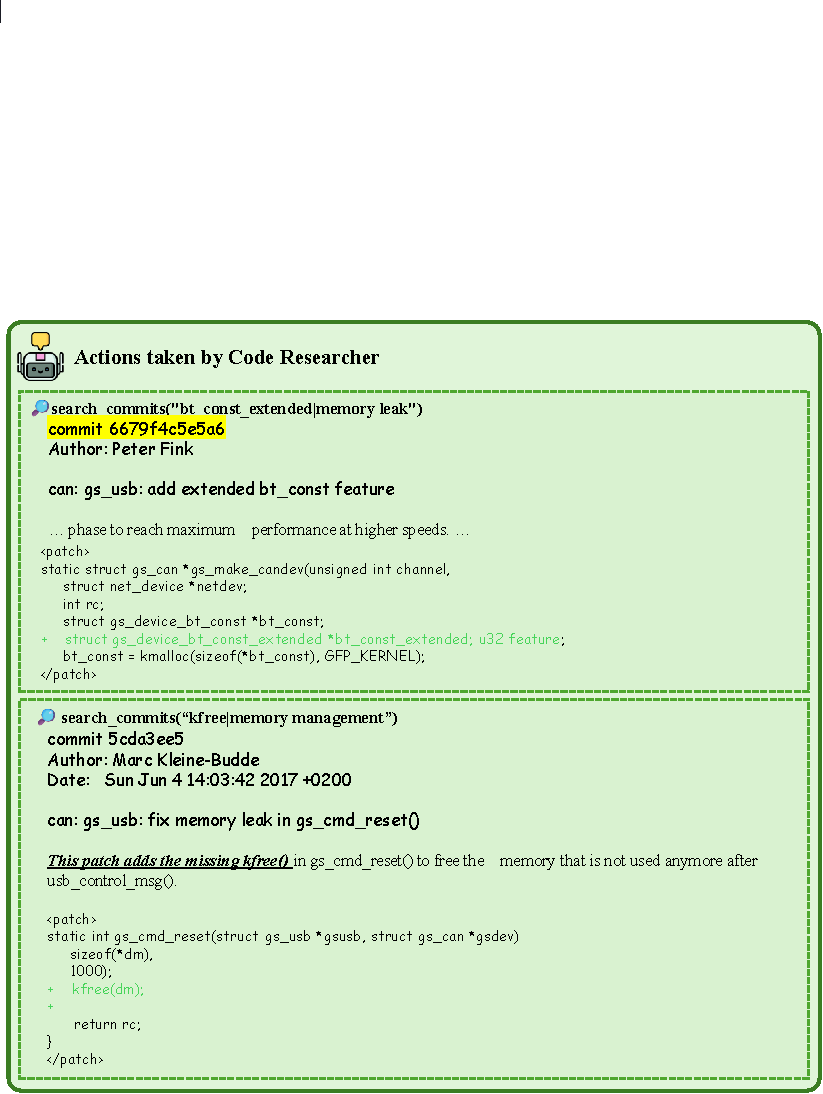
\includegraphics[width=\linewidth]{images/commit-importance-b.pdf}
    \caption{\cresearcher{} actions (\texttt{search\_commits} in green box).}
    \label{fig:code_b}
\end{figure}

\begin{figure}[H]
    \centering
    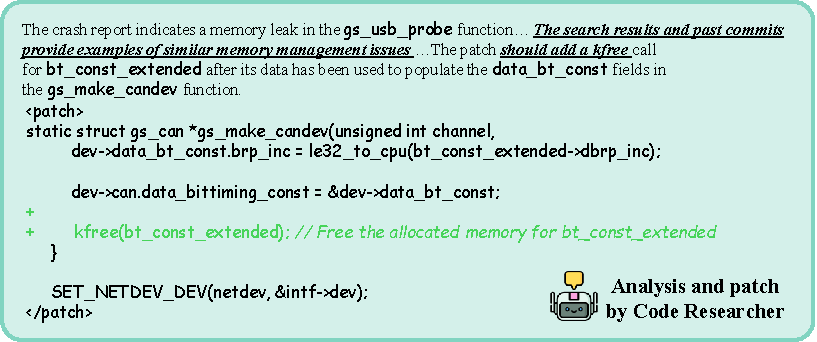
\includegraphics[width=\linewidth]{images/commit-importance-c.pdf}
    \caption{\cresearcher{} patch and analysis.}
    \label{fig:code_c}
\end{figure}